%%%%%%%%%%%%%%%%%%%%%%%%%%%%%%%%%%%%%%%%%
% University/School Laboratory Report
% LaTeX Template
% Version 3.1 (25/3/14)
%
% This template has been downloaded from:
% http://www.LaTeXTemplates.com
%
% Original author:
% Linux and Unix Users Group at Virginia Tech Wiki 
% (https://vtluug.org/wiki/Example_LaTeX_chem_lab_report)
%
% License:
% CC BY-NC-SA 3.0 (http://creativecommons.org/licenses/by-nc-sa/3.0/)
%
%%%%%%%%%%%%%%%%%%%%%%%%%%%%%%%%%%%%%%%%%

%----------------------------------------------------------------------------
%	PACKAGES AND DOCUMENT CONFIGURATIONS
%----------------------------------------------------------------------------

\documentclass{article}

%\usepackage{siunitx}
	% Provides the \SI{}{} and \si{} command for typesetting SI units
\usepackage{graphicx} 
	% Required for the inclusion of images
\graphicspath{ {LaTeX_Images/} }
	% Directory where images are imported from
\usepackage{amsmath} 
	% Required for some math elements 

\setlength\parindent{0pt} 
	% Removes all indentation from paragraphs

%\renewcommand{\labelenumi}{\alph{enumi}.} 
	% Make numbering in the enumerate environment by letter rather than 
	% number (e.g. %section 6)

%\usepackage{times} 
	% Uncomment to use the Times New Roman font

\renewcommand{\vec}[1]{\mathbf{#1}}
%\renewcommand{\textfraction}{0.05}

\usepackage{subfigure}
	% Place figures side by side

\usepackage{textcomp}

%----------------------------------------------------------------------------
%	ABSTRACT
%----------------------------------------------------------------------------

\begin{document}

\begin{abstract}
Throughout the latter half of this course on digital systems, we have learned 
to design sequential systems. In this project, we built a sequential system of 
a vending machine controller by going through the process of designing the 
system from the high-level specification to the final implementation. We 
defined the encoding schemes of the input and output, created the state 
diagram and state table, used K-maps to methodically obtain minimal OR-AND 
switching expressions, and implemnted and simulated the gate network on Vivado.
\end{abstract}

%----------------------------------------------------------------------------
%	FUNCTIONS OF THE CIRCUIT
%----------------------------------------------------------------------------

\section{Switching Functions of the Circuit}
This section shows minimal switching expressions in OR-AND form of the 
outputs and JK flip-flops. The corresponding schematics accompany those
expressions below.\\

\begin{equation*}
z_1 = (s_1)(s'_0 + x_1)(x_0)
\end{equation*}
\begin{figure}[h!]
\centering
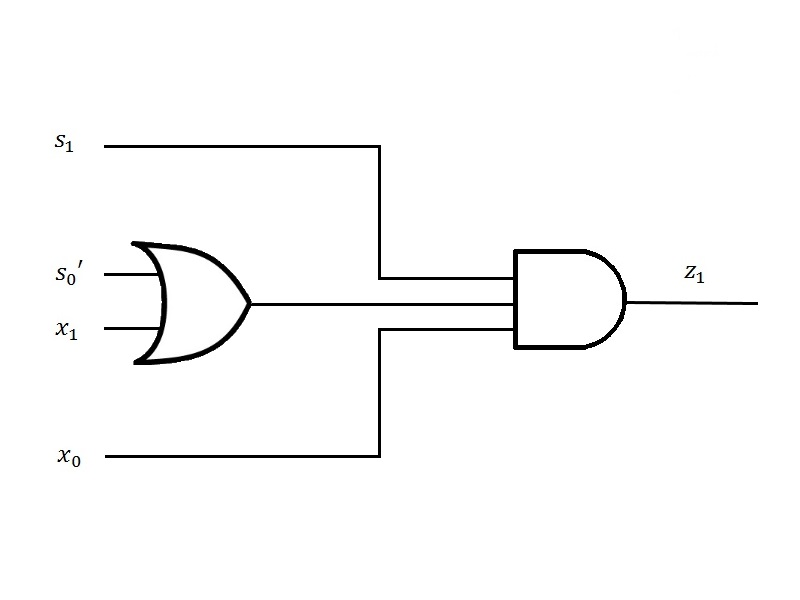
\includegraphics[scale=0.3]{z1}
\end{figure}

\clearpage

\begin{equation*}
z_0 = (s_1)(x_1)(s'_0)
\end{equation*}
\begin{figure}[h!]
\centering
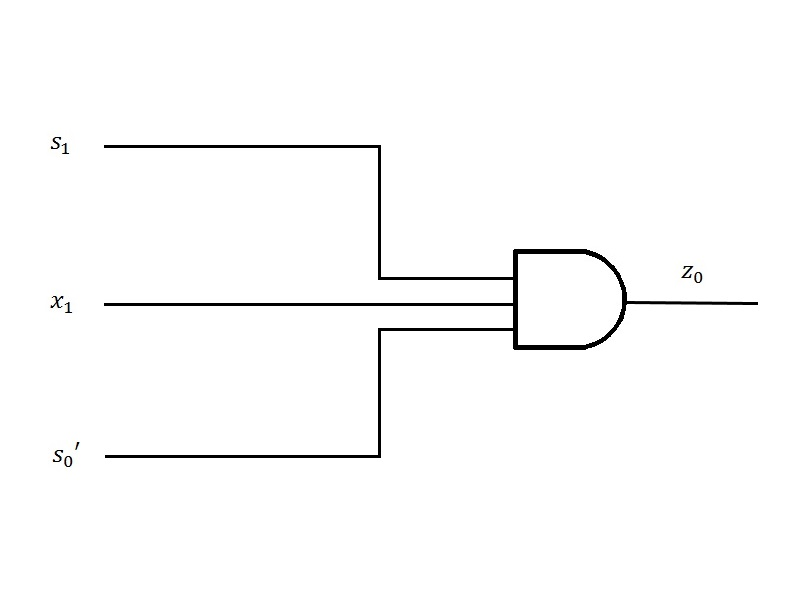
\includegraphics[scale=0.3]{z0}
\end{figure}

\begin{equation*}
J_1 = (x_0)(s_0 + x_1)
\end{equation*}
\begin{figure}[h!]
\centering
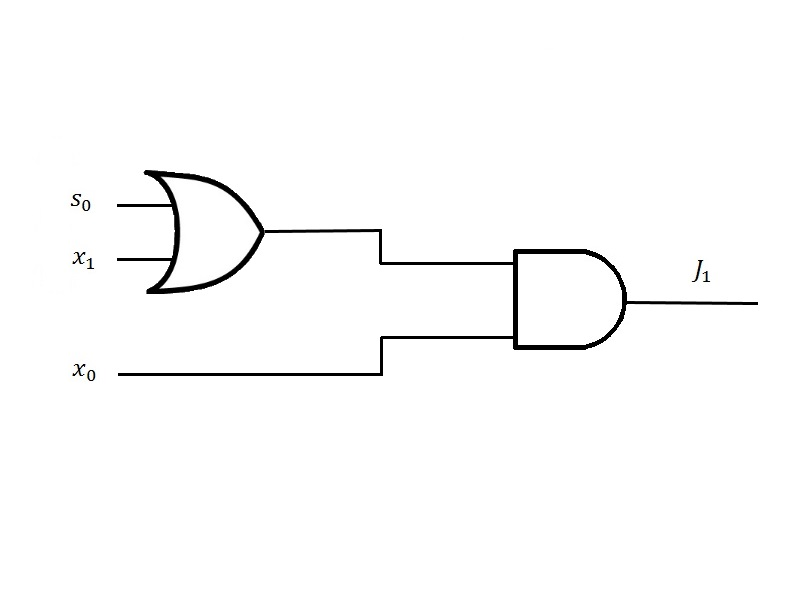
\includegraphics[scale=0.3]{J1}
\end{figure}

\clearpage

\begin{equation*}
K_1 = (x_0)(s'_0 + x_1)
\end{equation*}
\begin{figure}[h!]
\centering
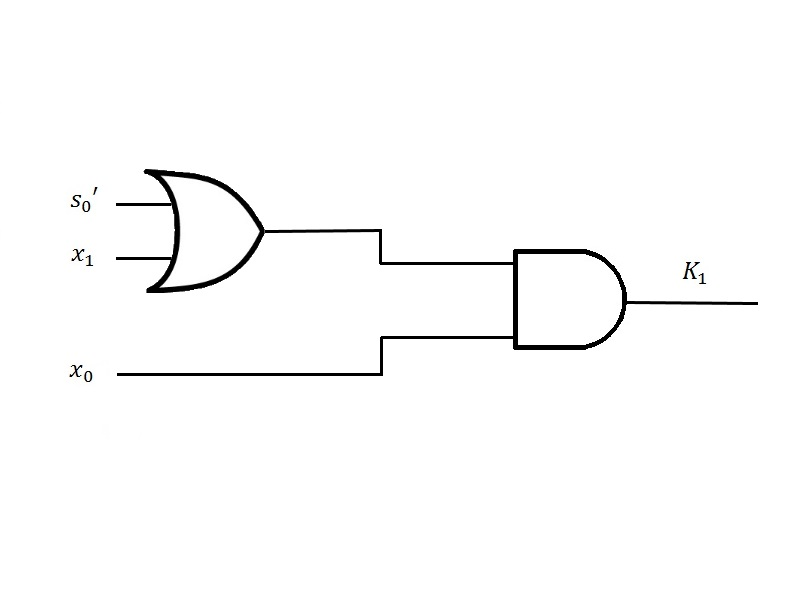
\includegraphics[scale=0.3]{K1}
\end{figure}

\begin{equation*}
J_0 = (s'_1)(x_0)
\end{equation*}
\begin{figure}[h!]
\centering
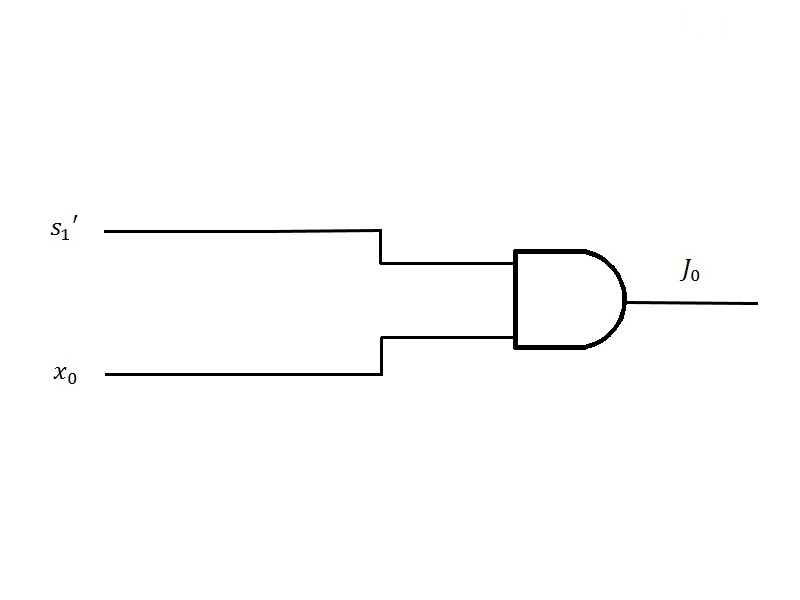
\includegraphics[scale=0.3]{J0}
\end{figure}

\clearpage

\begin{equation*}
K_0 = (x_0)(s_1 + x_1)
\end{equation*}
\begin{figure}[h!]
\centering
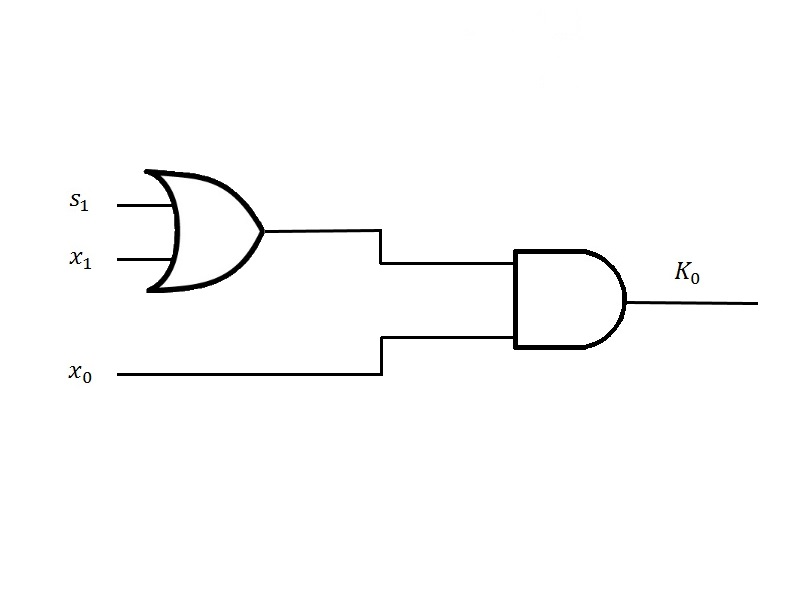
\includegraphics[scale=0.3]{K0}
\end{figure}

\textbf{We implemented negated inputs (of $s_0$ and $s_1$) using NOT gates as 
can be seen in the overall network in the Appendix.}
The same expressions can also be found in the Appendix. The Appendix gives a 
step-by-step procedure to obtain those expressions.

%----------------------------------------------------------------------------
%	VERILOG CODE
%----------------------------------------------------------------------------

\section{Verilog Code}
The following is the implementation of our circuit in code, pasted from a 
Verilog file. Please also refer to \textit{csm51a\_proj3.v} in the zipped 
file.

\begin{verbatim}
`timescale 1ns / 1ps
/////////////////////////////////////////////////////////////////////////////
// Company: UCLA Henry Samueli School of Engineering and Applied Science
// Engineers: Victor Lai and Dennis Gahm
// Student IDs: 404274720 and 704016107
// 
// Create Date: 05/27/2015 08:31:53 PM
// Design Name: 
// Module Name: csm51a_proj3
// Project Name: Verilog Lab #3
// Target Devices: 
// Tool Versions: 
// Description: 
// 
// Dependencies: 
// 
// Revision:
// Revision 0.01 - File Created
// Additional Comments:
// 
/////////////////////////////////////////////////////////////////////////////


module csm51a_proj3(x1, x0, clock, clear, z1,z0,pSout0, pSout1);
    input x1,x0,clock,clear;
    output z1,z0,pSout0, pSout1;
      
    wire[1:0] pS;
    wire[1:0] jk0_in;
    //reg jk00_in;
    wire[1:0] jk1_in;
    jkff jk0(pS[0], jk0_in, clock, clear);
    jkff jk1(pS[1], jk1_in, clock, clear);
    
    //combinational logic
    assign jk0_in[1] = x0 & ~pS[1];
    assign jk0_in[0] = x0 & (pS[1] | x1);
    //assign jk0_in2 = {x0 & ~pS[1], x0 & (pS[1] | x1)};
    assign jk1_in[1] = x0 & (pS[0] | x1);
    assign jk1_in[0] = x0 & (x1 | ~pS[0]);
    assign z0 = pS[1] & ~pS[0] & x1;
    assign z1 = x0 & pS[1] & (~pS[0] | x1);
    
    assign pSout0 = pS[0];
    assign pSout1 = pS[1];    
endmodule
\end{verbatim}

The Verilog code that follows shows our implementation of the JK flop-flop. 
Please also refer to \textit{jkff.v} in the zipped file.\\

\begin{verbatim}
`timescale 1ns / 1ps
/////////////////////////////////////////////////////////////////////////////
// Company: UCLA Henry Samueli School of Engineering and Applied Science
// Engineers: Victor Lai and Dennis Gahm
// Student IDs: 404274720 and 704016107 
// 
// Create Date: 05/28/2015 12:29:46 PM
// Design Name: 
// Module Name: jkff
// Project Name: Verilog Lab #3
// Target Devices: 
// Tool Versions: 
// Description: 
// 
// Dependencies: 
// 
// Revision:
// Revision 0.01 - File Created
// Additional Comments:
// 
/////////////////////////////////////////////////////////////////////////////


module jkff(data_out, data_in, clock, clear);
    output data_out;
    input[1:0] data_in;
    input clock, clear;
    reg[1:0] data_reg; //[1] is output/ps, [0] is next state/stored
    
    assign data_out = data_reg[0];
    
    always @(posedge clear or posedge clock)
    begin
        if (clear == 1)
            data_reg <= 0;
        else
            begin
                //data_out <= data_reg;
                if (data_reg[0] == 0)
                    begin
                        if (data_in[1] == 1)
                        begin
                            data_reg[1] = data_reg[0];
                            data_reg[0] = 1;
                        end
                    end
                else
                    begin
                        if (data_in[0] == 1)
                            data_reg[1] = data_reg[0];
                            data_reg[0] = 0;
                    end
            end 
    end

endmodule
\end{verbatim}

%----------------------------------------------------------------------------
%	SIMULATION RESULT
%----------------------------------------------------------------------------

\section{Simulation Result}
We simulated three sequences: (1) D, N, D; (2) N, N, N, N, and (3) D, Reset.\\
\\
Figure~\ref{fig:dnd} shows the simulation of the sequence of D, N, D. Going 
from left to right, we see that the input \textit{clear} for the two JK 
flip-flops are set, causing the flip flops to store 0 (indicated by 
\textit{psOut0} and \textit{psOut1}). In addition, the moment that 
\textit{clear} is 1, the flip-flops store 0 regardless of the clock because 
that input is asynchronous. When the dime comes in as input (when $x_1=1$ and 
$x_0=1$), on the positive edge of the clock the flip-flops' state changes to 
11, which represents the state for 10\textcent. Then, a nickel is input (when 
$x_1=0$ and $x_0=1$), and the state changes to 10, which represents the state 
for 15\textcent. Finally, when a dime is inserted as input, the state changes to 
00 (0 cents or initial state) and $z_1=1$ and $z_0=1$ on the positive edge of 
the clock (because it is synchronous), which represents the output for 
releasing gum and releasing a nickel as change since the gum is 20\textcent.

\clearpage

\begin{figure}[h!]
\centering
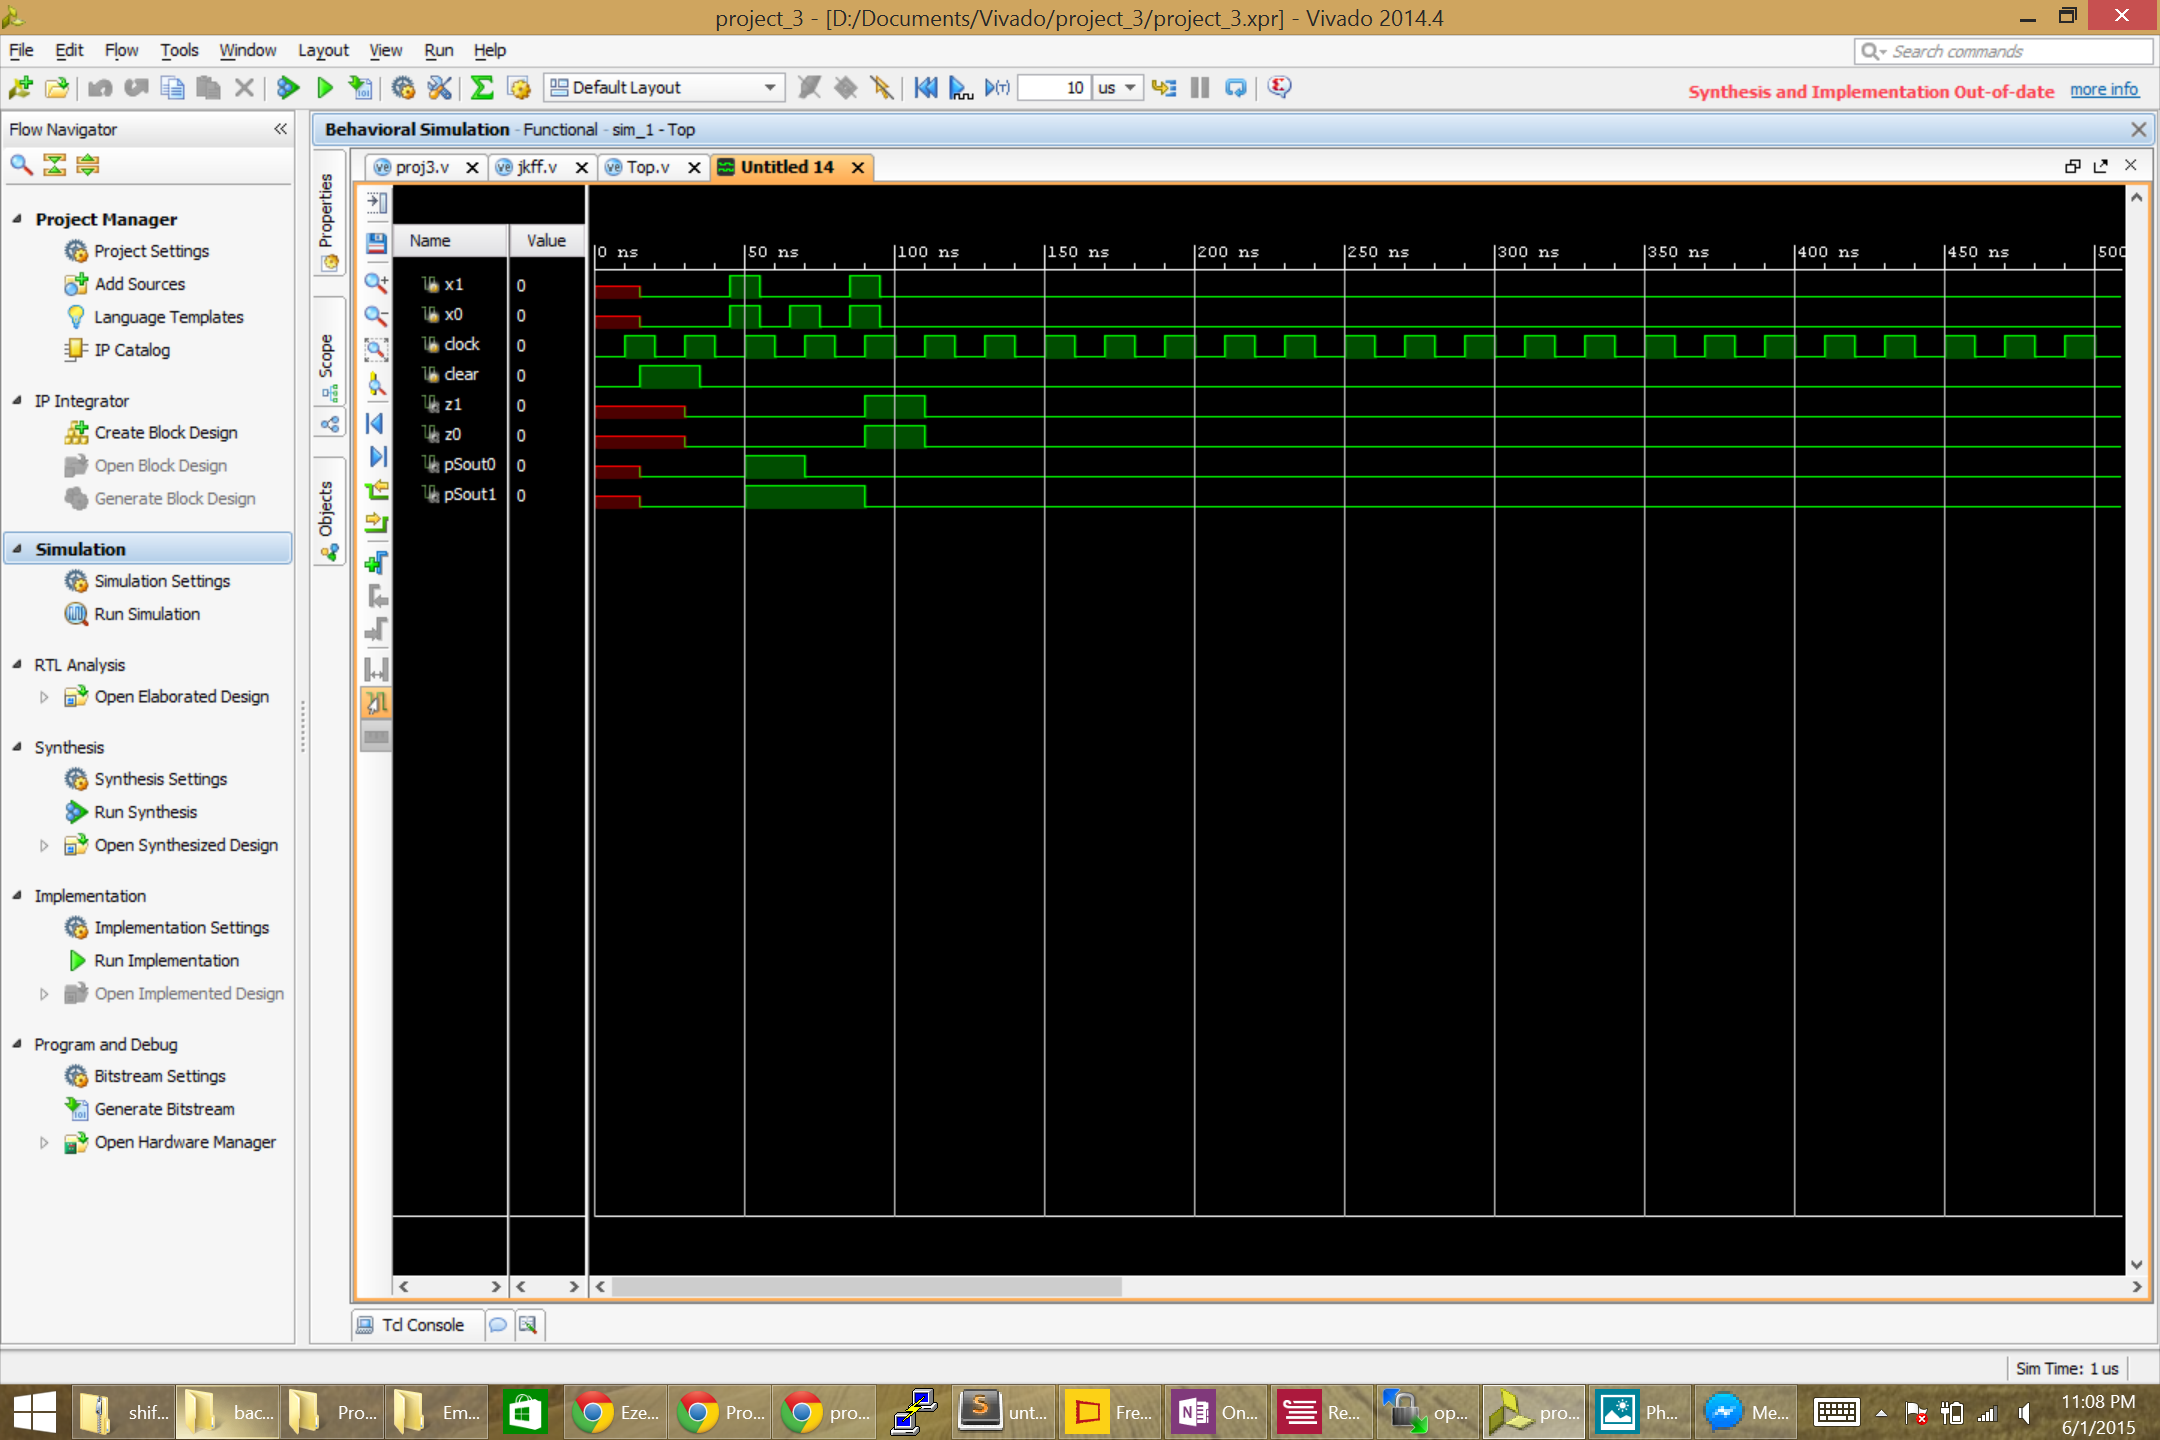
\includegraphics[scale=0.4]{DND}
\caption{The full screen result of the simulation for D, N, D in Vivado}
\label{fig:dnd}
\end{figure}

Figure~\ref{fig:nnnn} shows ths simulation of the sequence of four nickels. 
Similarly, we set the \textit{clear} input in order to set the two flip-flops 
to 0. Four nickels are inserted as input, each changing the state of the 
flip-flops.  When the fourth nickel is inserted, $z_1$ becomes 1 and $z_0=0$ 
because the gum is released and a nickel is not returned as expected since 
exactly 20\textcent was taken and the gum costs 20\textcent. 

\clearpage

\begin{figure}[h!]
\centering
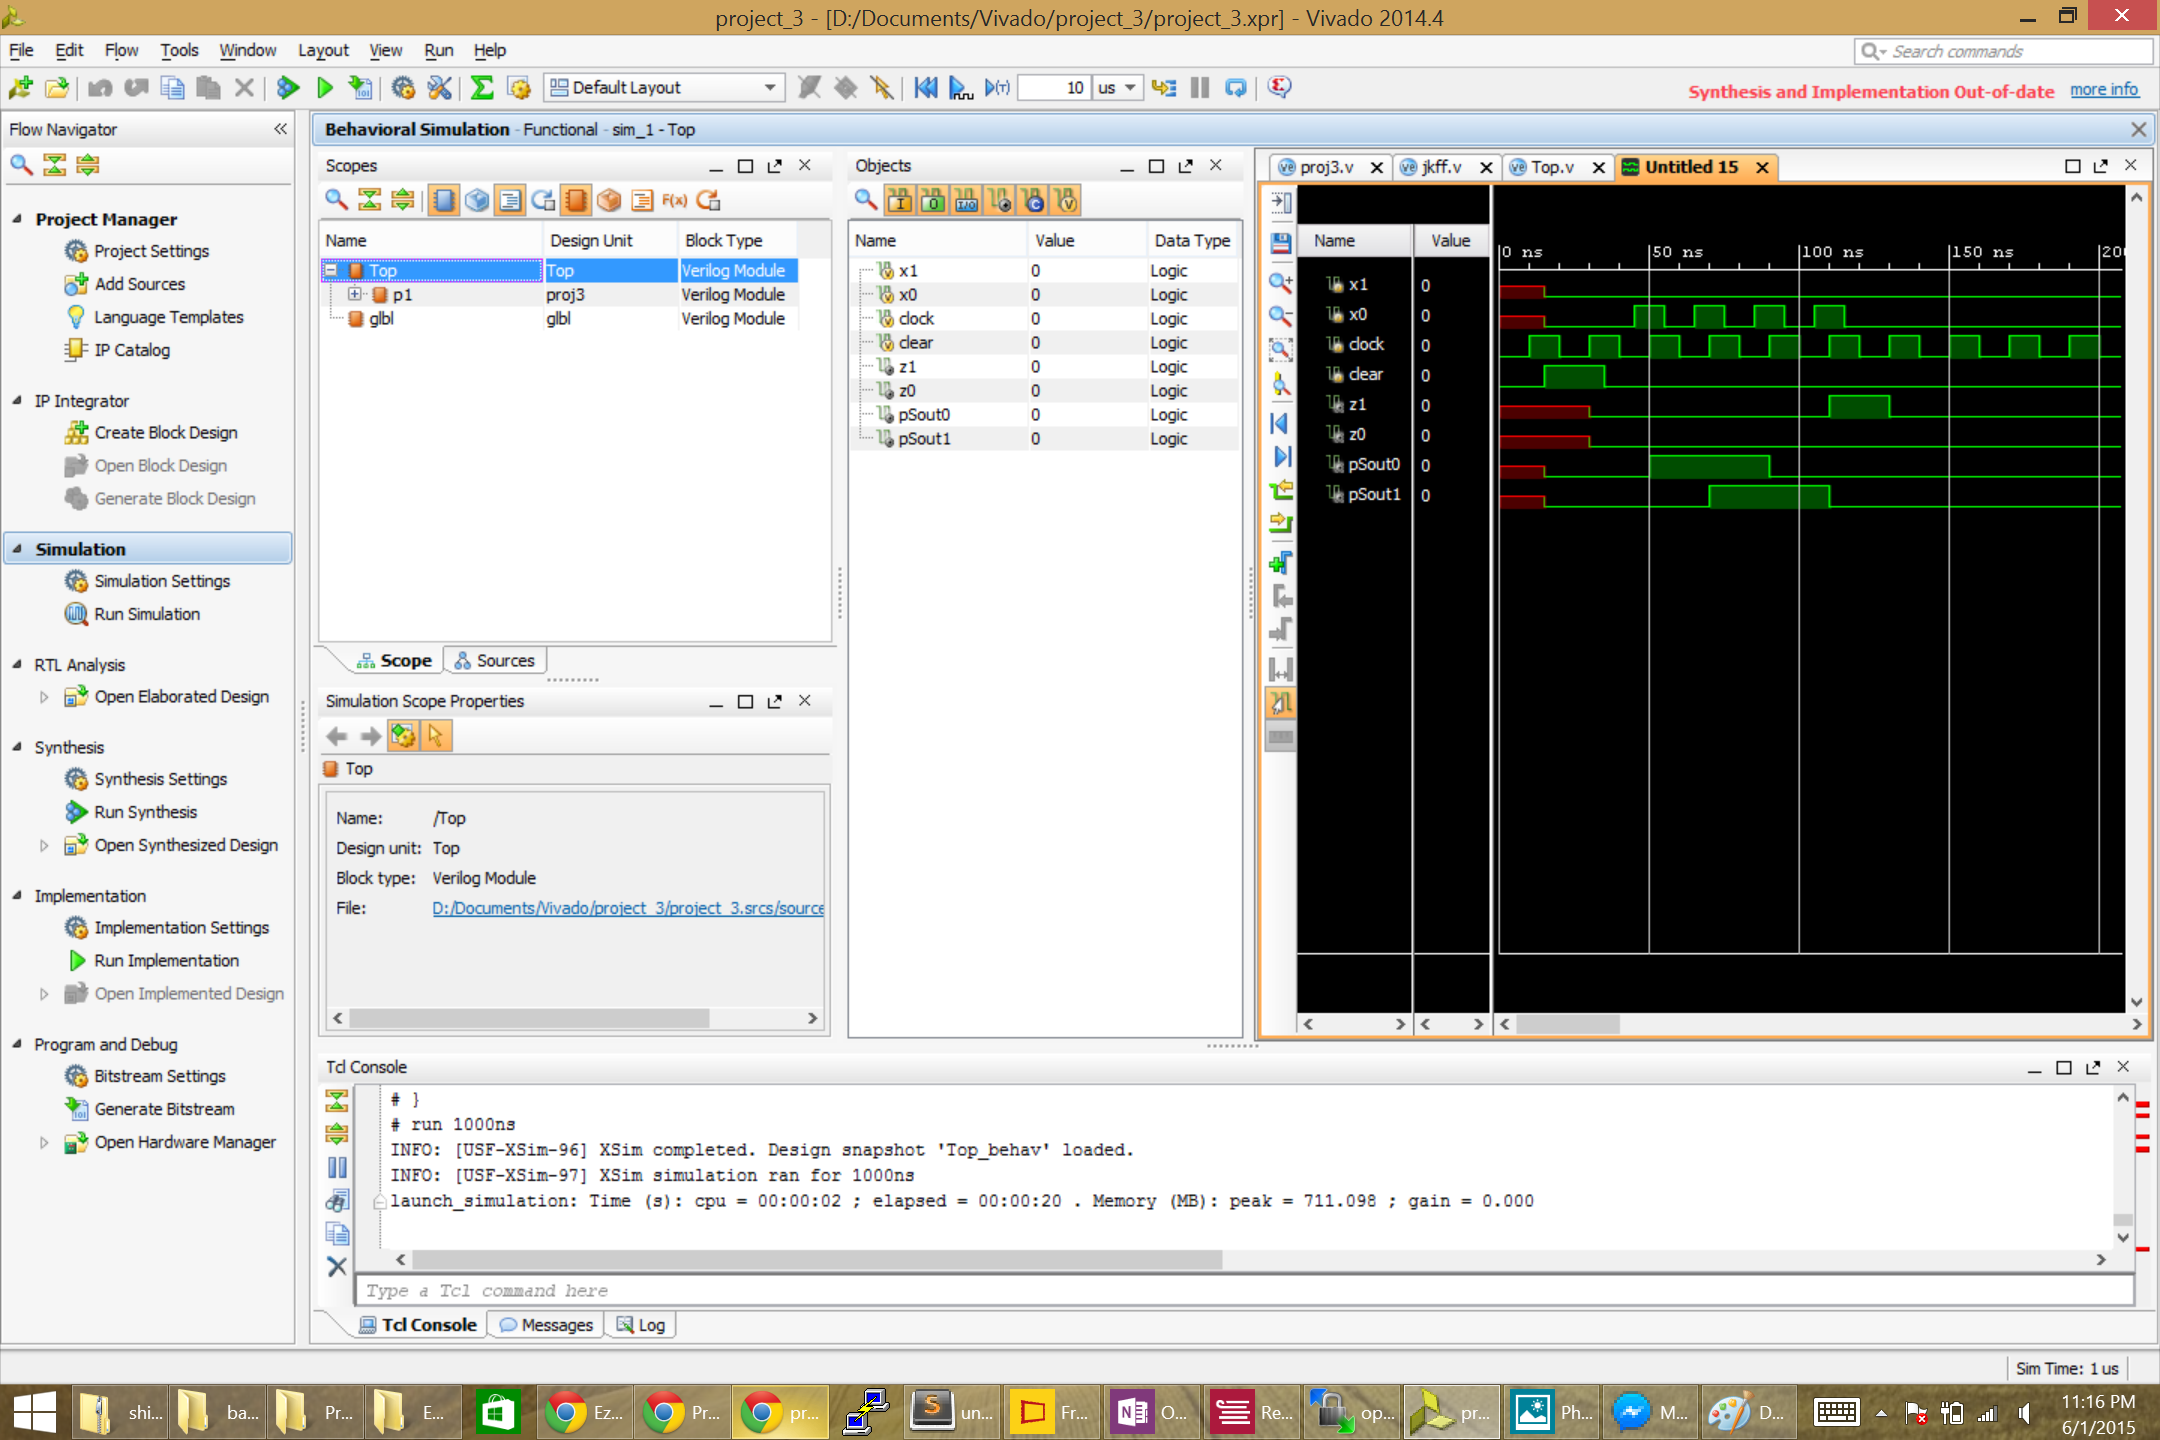
\includegraphics[scale=0.4]{NNNN}
\caption{The full screen result of the simulation for N, N, N, N in Vivado}
\label{fig:nnnn}
\end{figure}

In Figure~\ref{fig:d_reset}, we show the sequence of D, Reset in another 
simulation. We set the input \textit{clear} as usual before inserting a dime as 
input and then setting \textit{clear} to siginify a reset. As with the first 
\textit{clear} input, the \textit{clear} input asychronously and immediately 
sets the flip-flops to 00.

\clearpage

\begin{figure}[h!]
\centering
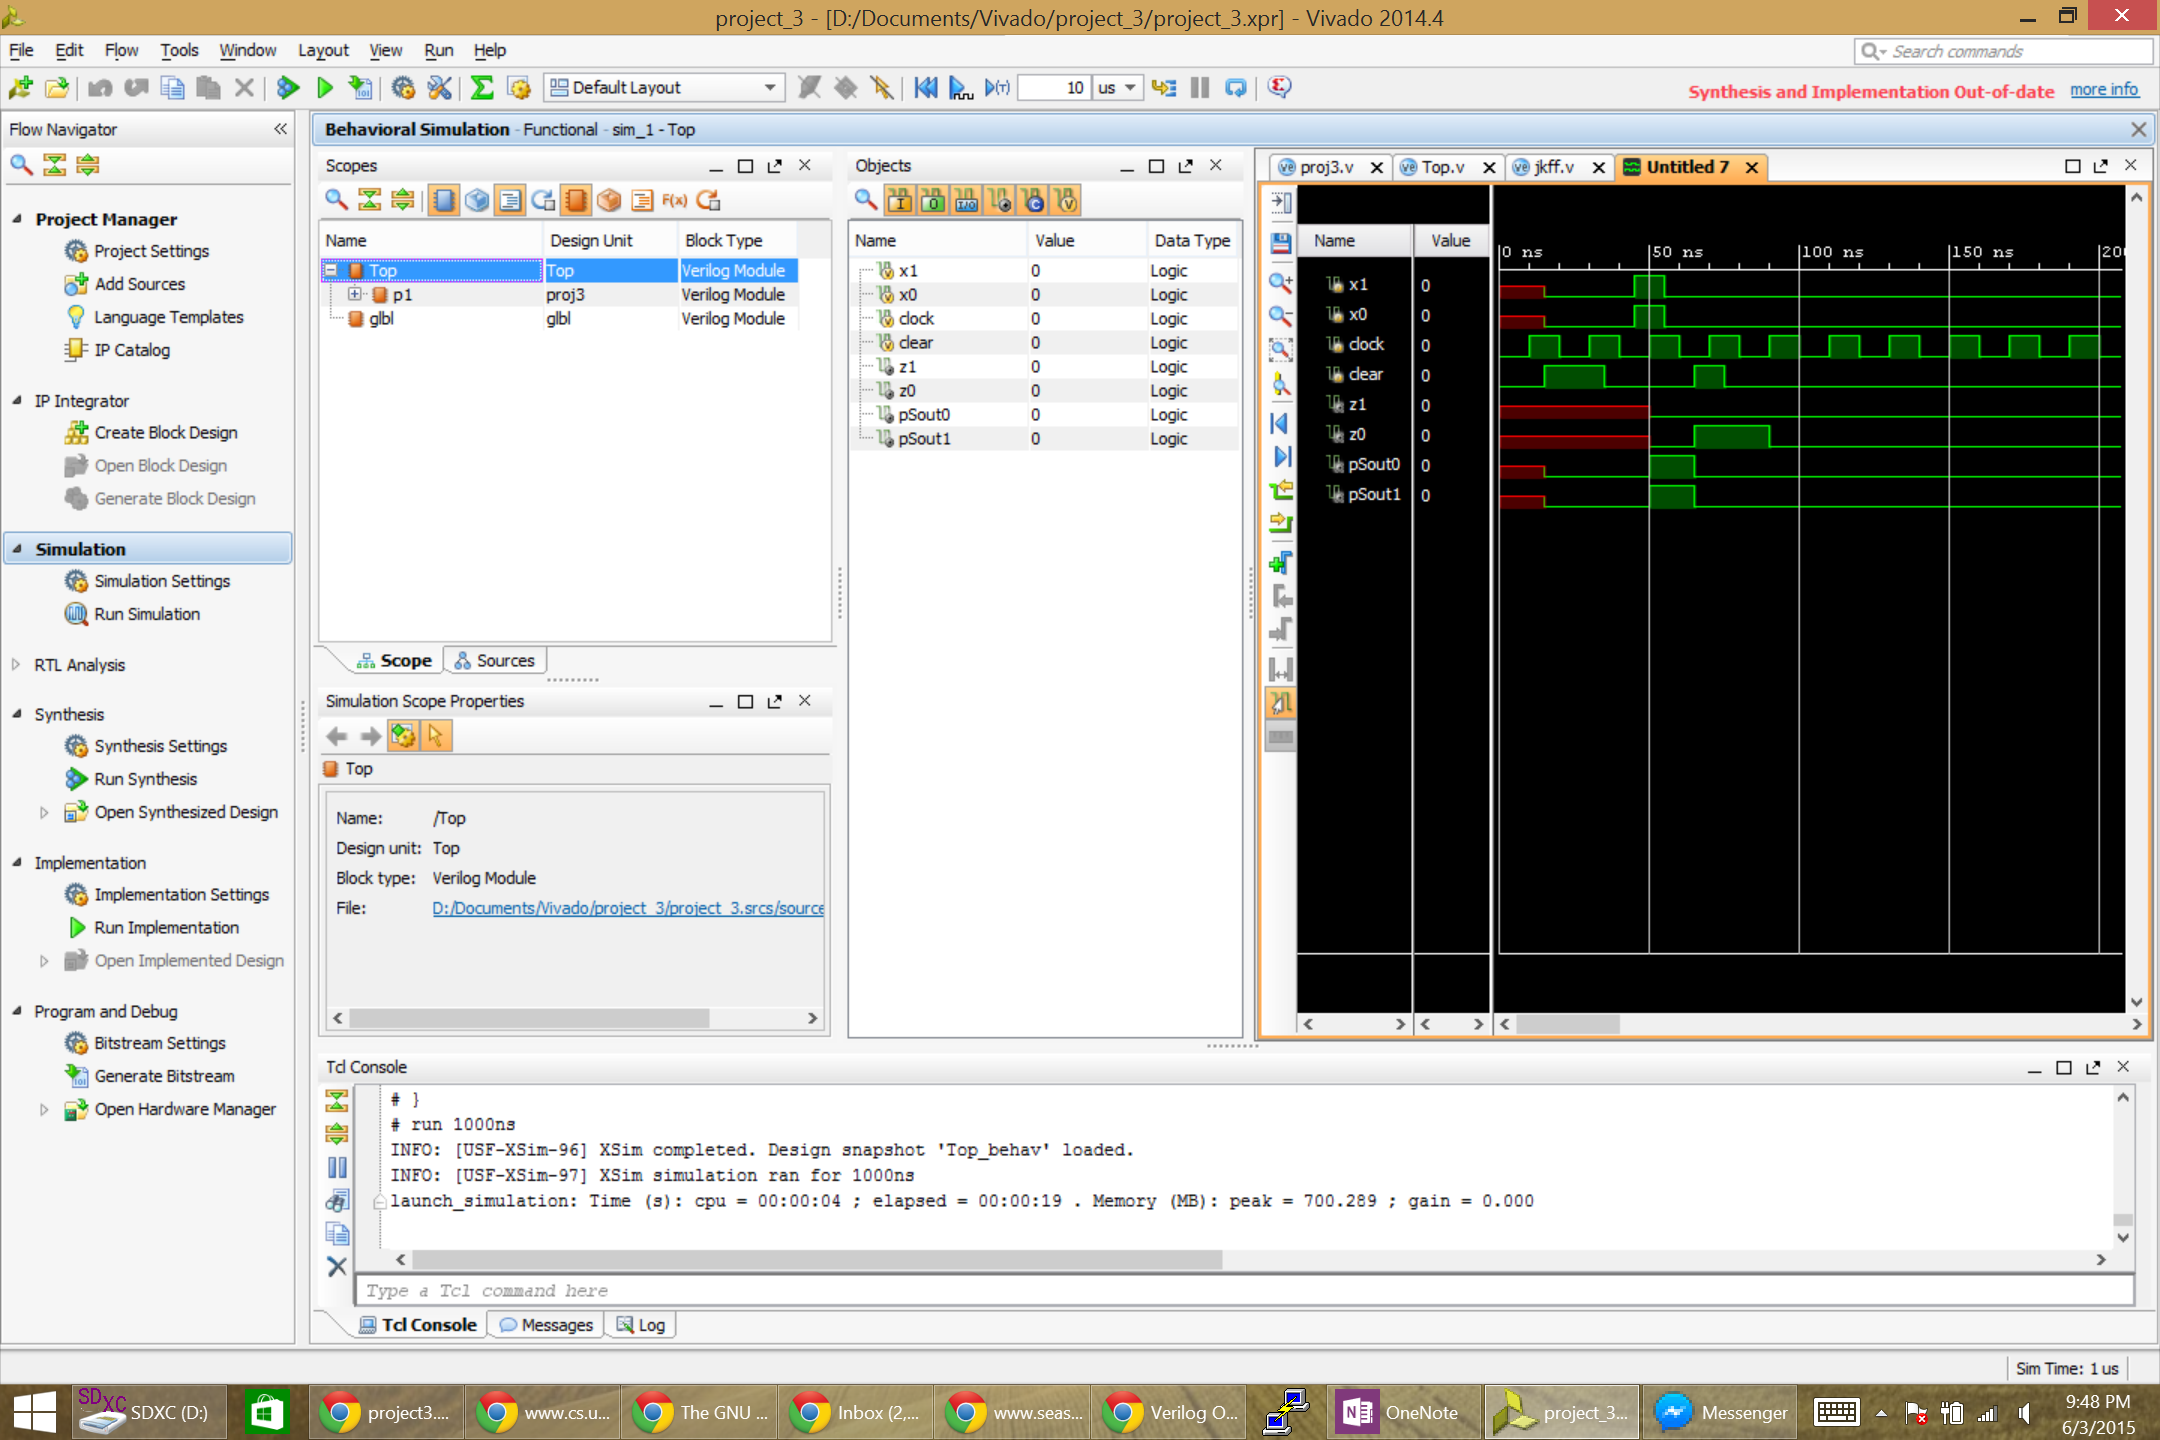
\includegraphics[scale=0.4]{D_Reset}
\caption{The full screen result of the simulation for D, Reset in Vivado}
\label{fig:d_reset}
\end{figure}

The following test bench code was used to generate those simulation results.

\begin{verbatim}
`timescale 1ns / 1ps
/////////////////////////////////////////////////////////////////////////////
// Company: UCLA Henry Samueli School of Engineering and Applied Science
// Engineers: Victor Lai and Dennis Gahm
// Student IDs: 404274720 and 704016107
// 
// Create Date: 05/28/2015 01:39:02 PM
// Design Name: 
// Module Name: csm51a_proj3_tb.v
// Project Name: Verilog Lab #3
// Target Devices: 
// Tool Versions: 
// Description: 
// 
// Dependencies: 
// 
// Revision:
// Revision 0.01 - File Created
// Additional Comments:
// 
/////////////////////////////////////////////////////////////////////////////


module Top;
    reg x1,x0,clock,clear;
    wire z1, z0,pSout0,pSout1;
    csm51a_proj3 p1(x1, x0, clock, clear, z1,z0,pSout0, pSout1);
    
    initial begin
        clock = 0;
        clear = 0;
        #15 clear = 1; x1=0;x0=0;
        #20 clear = 0;
        #10 x1=0;x0=1;
    end
    
    always begin
        #10 clock = ~clock;
    end
endmodule

\end{verbatim}

%----------------------------------------------------------------------------
%	DESIGN REVIEW
%----------------------------------------------------------------------------

\section{Design Review}
Throughout the process of completing this project, we learned many things 
ranging from applying concepts that we learned in class to getting more 
comfortable using new software.\\
\\
In this project, we learned how to apply the concepts of sequential systems 
which we learned in class to a real-world application. In particular, we 
learned that a vending machine functions as a sequential system in that it 
keeps track of the coins that are inserted and appropriately releases the item 
when enough coins have been put in.\\
\\
Having practiced the techinques often in class, we found that getting the 
minimal switching expressions was nearly trivial to do.\\
\\
Implementing our design in Vivado turned out to be very difficult, and most of 
our time was spent getting the simulation results to be correct as a result. 
We think that the instructor and/or teaching assistants could have spent a bit 
more time discussing the Verilog syntax of sequential systems in general.\\
\\
If we had more time, we would have attempted to do the extra credit and 
implemented another design using multiplexers. If we did not have any trouble 
implementing our design in Vivado, then we could have possibly worked on 
designing a controller that also accepts quarters.

%----------------------------------------------------------------------------
%	TEAM MEMBER CONTRIBUTIONS
%----------------------------------------------------------------------------

\section{Team Member Contributions}
Each team member assumed a relatively equal share of the workload of this 
project.\\
\\
Dennis mainly worked on the technical aspect of this project. He spend most of 
his time trying to correctly implement our design in Verilog. Part of that time 
involved going to office hours to verify that the implemented code is flawless. 
He also checked Victor's initial design done on paper and was able to catch a 
few mistakes. \\
\\
Victor mostly worked on the compilation of the report using \LaTeX. He created 
the individual gate networks as well as the final network of gates and 
flip-flops using Paint. The pencil-and-paper design in Section 6.6 shows his 
work which was later verified by Dennis. He also wrote out most of the text of 
the report.\\
\\
Overall, each member of the team contributed to roughly 50\% to the completion 
of the project.

%----------------------------------------------------------------------------
%	APPENDIX
%----------------------------------------------------------------------------

\section{Appendix}
This part must show the complete worksheet during the paper-and-paper design.

\subsection{Inputs, Outputs, and States of the System}
Professor Yutao He always reminds his students to draw "The Box" when starting 
to design and analyze a digital system. Remembering that piece of advice, we 
started our design by drawing it to get a sense of the inputs and outputs. 
Those inputs and outputs are depicted in Figure~\ref{fig:box}. \\

\clearpage

\begin{figure}[h!]
\centering
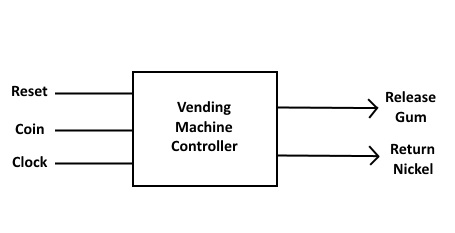
\includegraphics[scale=0.7]{Box}
\caption{"The Box!"}
\label{fig:box}
\end{figure}

The following tables show the inputs, outputs, and states of the \textit{iKon} 
Controller.

\begin{table}[h]
\begin{center}
\begin{tabular}{|c|c|c|c|l}
\cline{1-4}
\multicolumn{2}{|c|}{ \textbf{Inputs} } & 
\multicolumn{2}{c|}{ \textbf{Outputs} } &  \\ \cline{1-4}
  \textbf{Variables} & \textbf{Values} & \textbf{Variables} & \textbf{Values} &
  \\ \cline{1-4}
  Reset & \{True (T), False (F)\} & Release Gum (RG) & \{T, F\} &  \\
  Coin & \{ Empty (E), Nickel (N), Dime (D) \} & Return Nickel (RN) & \{T, F\} 
  &  \\ \cline{1-4}
\end{tabular}
\caption{The Inputs and Outputs of the \textit{iKon} Controller}
\end{center}
\end{table}

\begin{table}[h]
\begin{center}
\begin{tabular}{|c|c|}
\hline
\textbf{State} & \textbf{Description}                  \\ \hline
Init           & Initial State                         \\
5c             & Amount of deposited coins is 5\textcent  \\
10c            & Amount of deposited coins is 10\textcent \\
15c            & Amount of deposited coins is 15\textcent \\ \hline
\end{tabular}
\caption{The States of the \textit{iKon} Controller}
\end{center}
\end{table}


\subsection{Encoding Schemes}
Thee following tables show the encoding schemes that we used to design the 
sequential network.

\clearpage

\begin{table}[h]
\begin{center}
\begin{tabular}{cc|cc}
\textbf{Coin} & $x_1$$x_0$ & \textbf{Reset}       & r                \\ \hline
Empty         & 00   & False                & 0                    \\
Nickel        & 01   & True                 & 1                    \\
Dime          & 11   & \multicolumn{1}{l}{} & \multicolumn{1}{l}{}
\end{tabular}
\caption{The Encoding Scheme of the Inputs}
\end{center}
\end{table}

\begin{table}[h]
\begin{center}
\begin{tabular}{cc|cc}
\textbf{RG} & $z_1$ & \textbf{RN} & $z_0$ \\ \hline
False       & 0  & False       & 0  \\
True        & 1  & True        & 1 
\end{tabular}
\caption{The Encoding Scheme of the Outputs}
\end{center}
\end{table}

\begin{table}[h]
\begin{center}
\begin{tabular}{c|c}
\textbf{State} & $s1$$s0$ \\ \hline
Init           & 11   \\
5c             & 01   \\
10c            & 11   \\
15c            & 10  
\end{tabular}
\caption{The Encoding Scheme of the States}
\end{center}
\end{table}


\subsection{State Diagram and State Table}
The following is the state diagram.

\clearpage

\begin{figure}[h!]
\centering
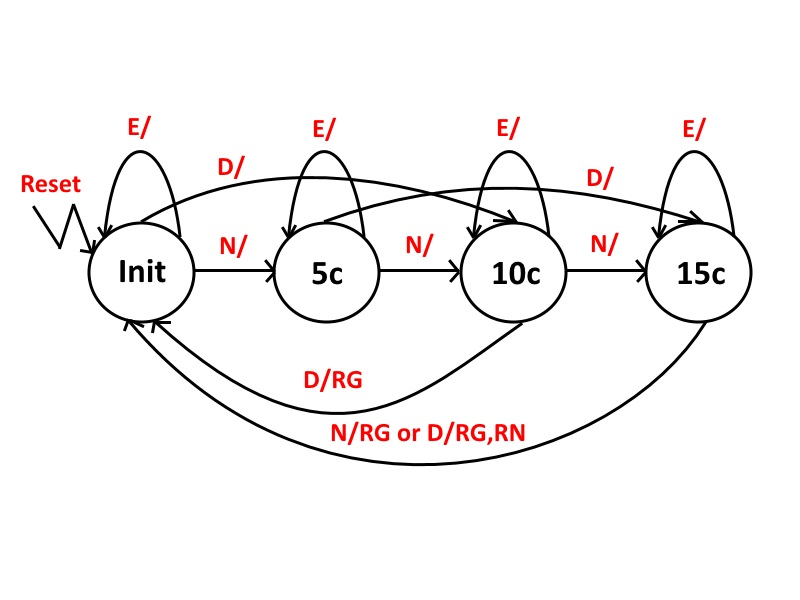
\includegraphics[scale=0.5]{State_Diagram}
\caption{The State Diagram of the Controller}
\end{figure}

The following is the state table obtained from the state diagram.

\begin{table}[h]\
\begin{center}
\begin{tabular}{c|ccc}
PS  & \multicolumn{3}{c}{ 
  \begin{tabular}[c]{@{}c@{}} Input \\ $x_1$$x_0$ 
  \end{tabular} 
} \\ \hline
s(t) = $s_1$$s_0$  & 00              & 01               & 11    \\ \hline
00                 & 00, 00          & 01, 00           & 11, 00\\
01                 & 01, 00          & 11, 00           & 10, 00\\
11                 & 11, 00          & 10, 00           & 00, 10\\
10                 & 10, 00          & 00, 10           & 00, 11\\ \hline
\multicolumn{1}{l|}{} & \multicolumn{3}{c}{
  \begin{tabular}[c]{@{}c@{}} NS, Output\\ s(t + 1), z = $z_1$$z_0$
  \end{tabular}
}
\end{tabular}
\caption{The State Table of the Controller}
\end{center}
\end{table}


\subsection{Minimization Procedure}
We used K-maps to find the minimal product of sums. The red circles in the 
K-maps shown below indicate the implicates used in the minimal expressions.\\

\begin{table}[h!]
\begin{tabular}{ c c }
\centering
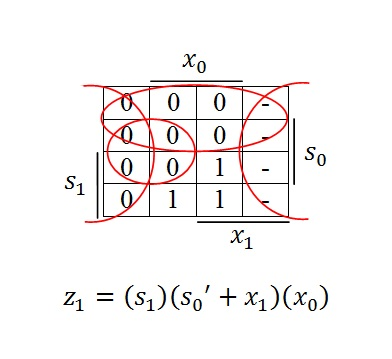
\includegraphics[scale=0.6]{z1-KMap} &
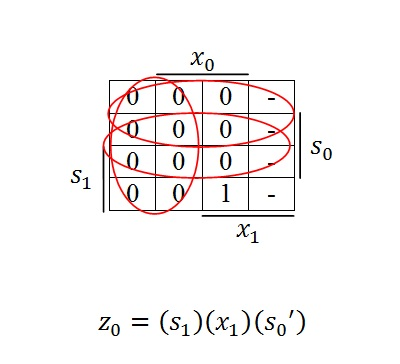
\includegraphics[scale=0.6]{z0-KMap} \\
\end{tabular}
\end{table}

\pagebreak

\begin{table}[h!]
\begin{tabular}{ c c }
\centering
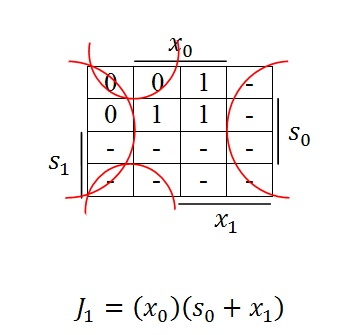
\includegraphics[scale=0.6]{J1-KMap} &
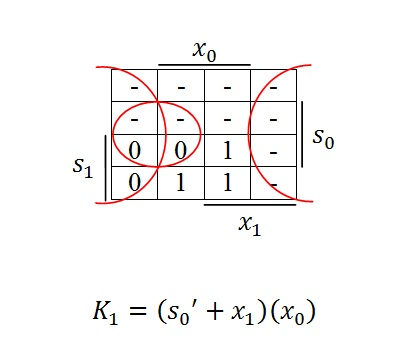
\includegraphics[scale=0.6]{K1-KMap} \\
\end{tabular}
\end{table}

\begin{table}[h!]
\begin{tabular}{ c c }
\centering
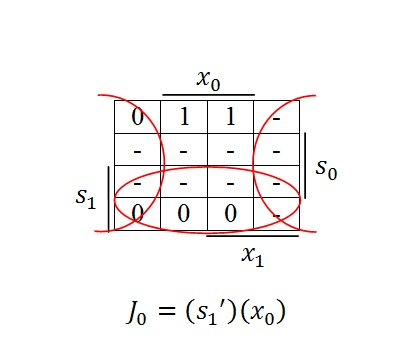
\includegraphics[scale=0.6]{J0-KMap} &
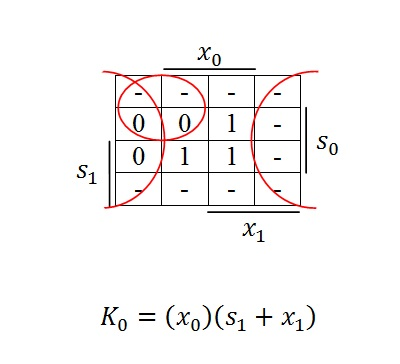
\includegraphics[scale=0.6]{K0-KMap} \\
\end{tabular}
\end{table}

\pagebreak


\subsection{Final Minimal Expressions}
After drawing the K-maps (from the previous section), we got the following 
minimal switching expressions in OR-AND form.\\

\begin{equation*}
z_1 = (s_1)(s'_0 + x_1)(x_0)
\end{equation*}

\begin{equation*}
z_1 = (s_1)(x_1)(s'_0)
\end{equation*}

\begin{equation*}
J_1 = (x_0)(s_0 + x_1)
\end{equation*}

\begin{equation*}
K_1 = (x_0)(s'_0 + x_1)
\end{equation*}

\begin{equation*}
J_0 = (s'_1)(x_0)
\end{equation*}

\begin{equation*}
K_0 = (x_0)(s_1 + x_1)
\end{equation*}

Combining each individual subnetwork of logic gates, we get the following 
circuit design.

\clearpage

\begin{figure}[h!]
\centering
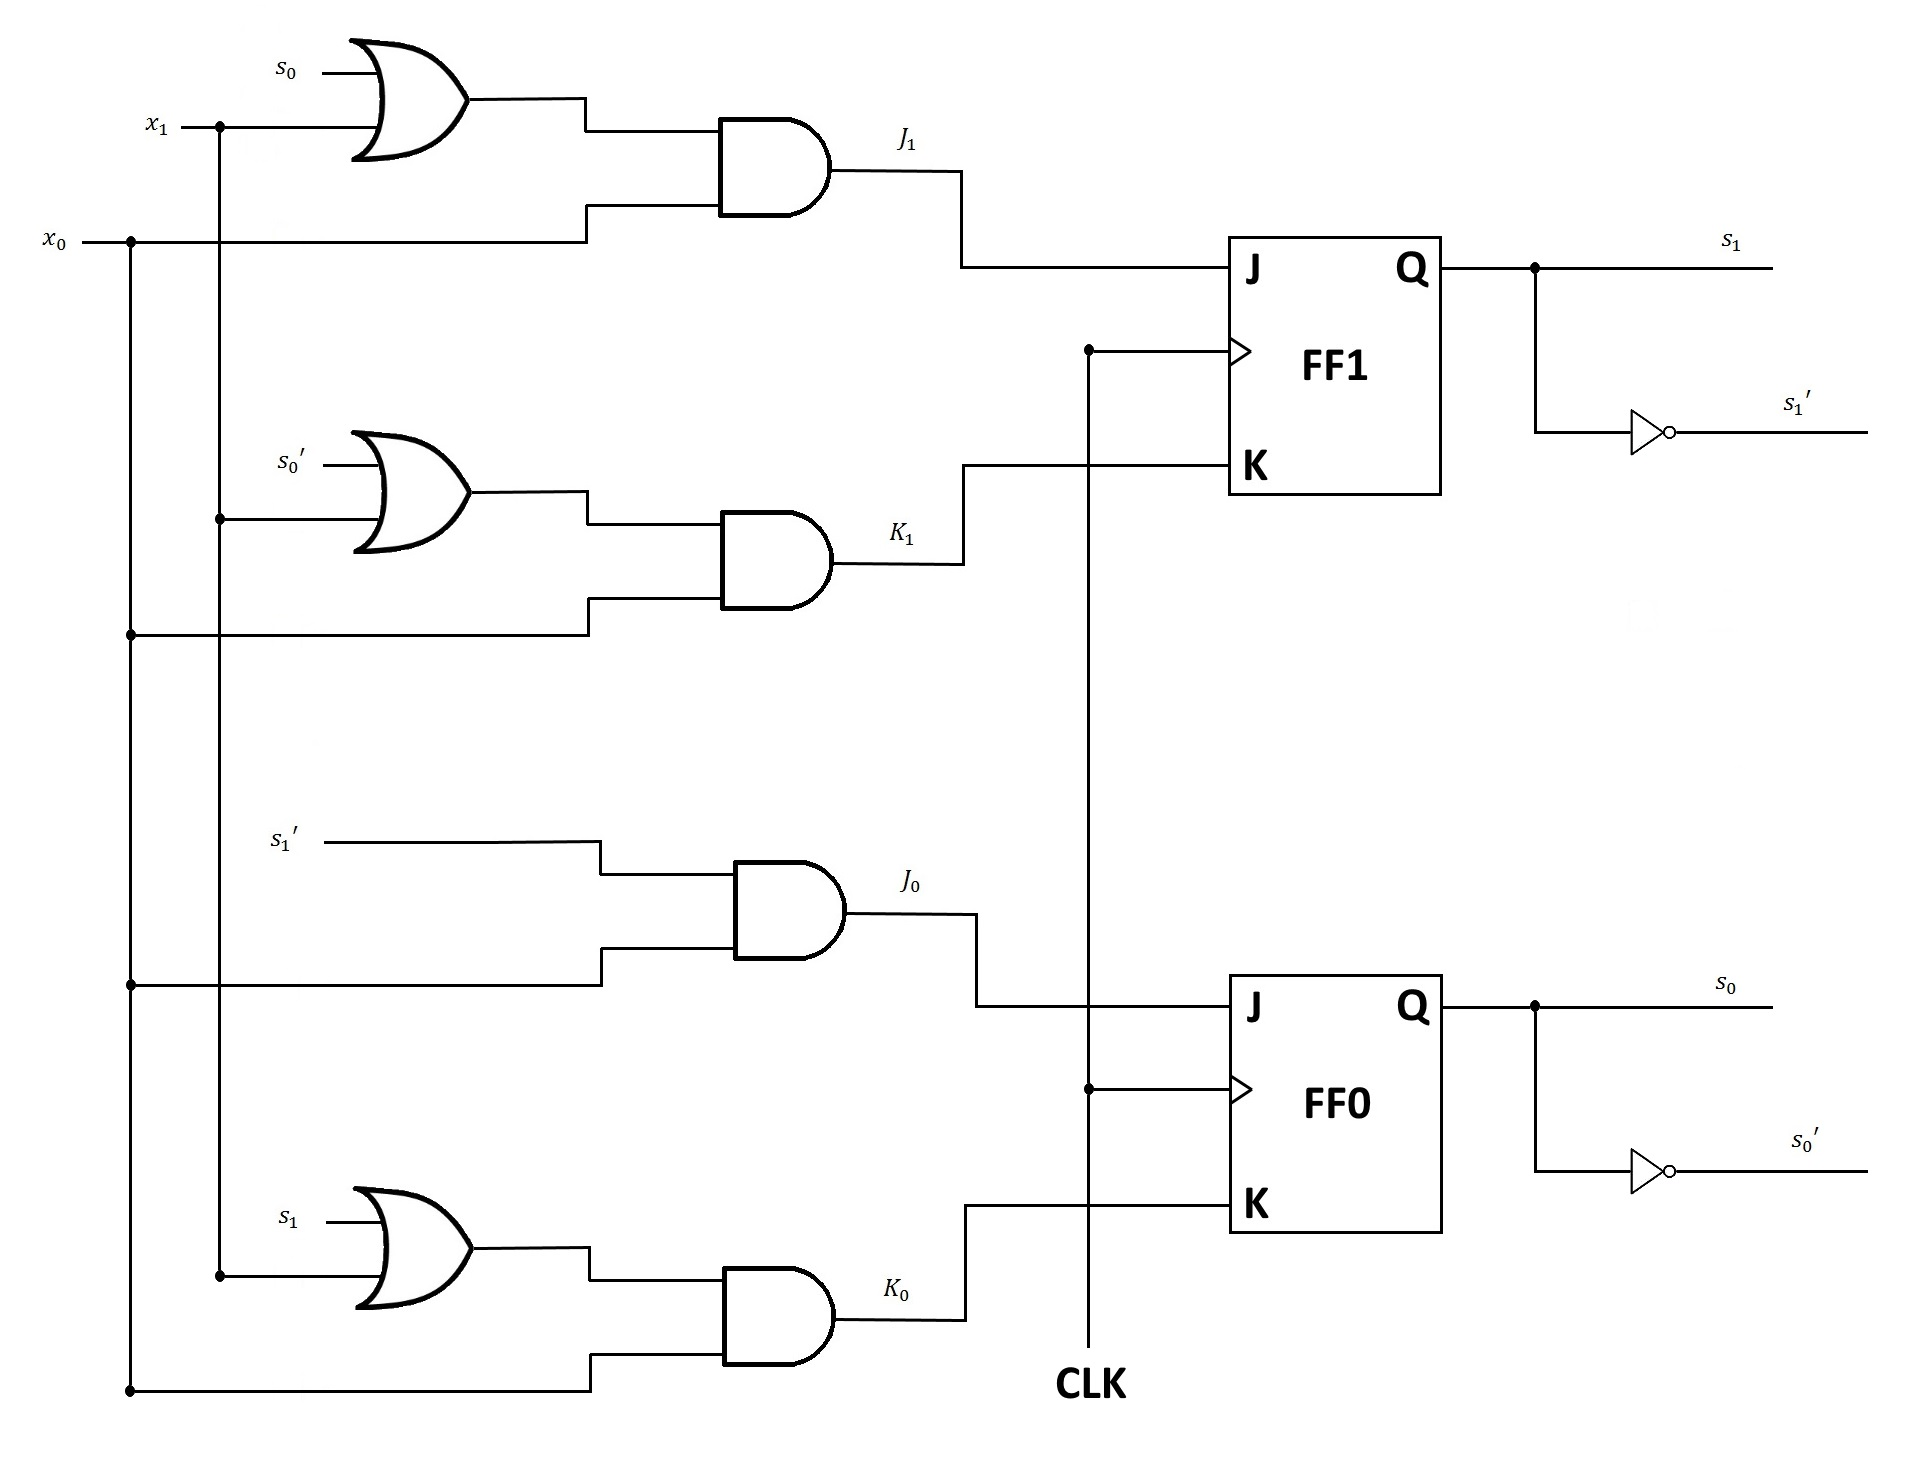
\includegraphics[scale=0.3]{Network}
\end{figure}

\begin{table}[h!]
\begin{tabular}{ c c }
\centering
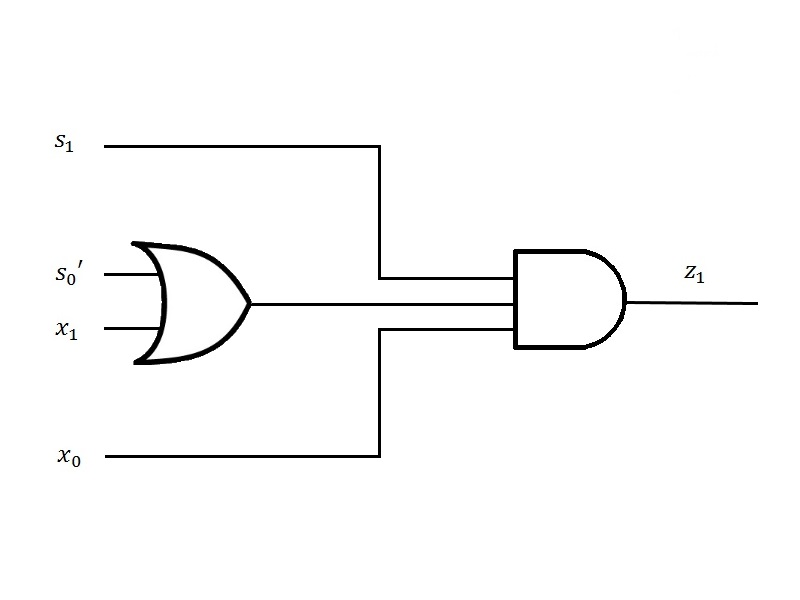
\includegraphics[scale=0.3]{z1} &
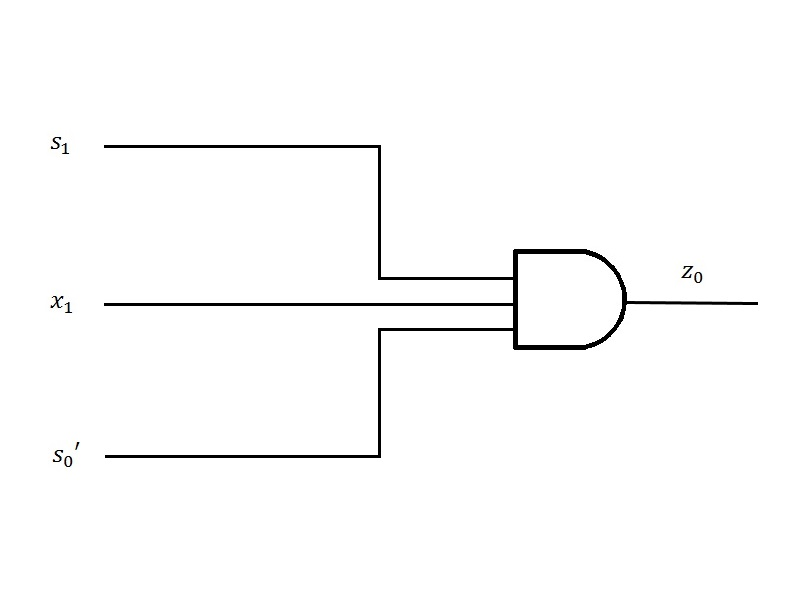
\includegraphics[scale=0.3]{z0} \\
\end{tabular}
\end{table}


\subsection{Paper-and-Pencil Design}
The following screenshots show our preliminary work done using paper and 
pencil.\\
\begin{figure}[h!]
\centering
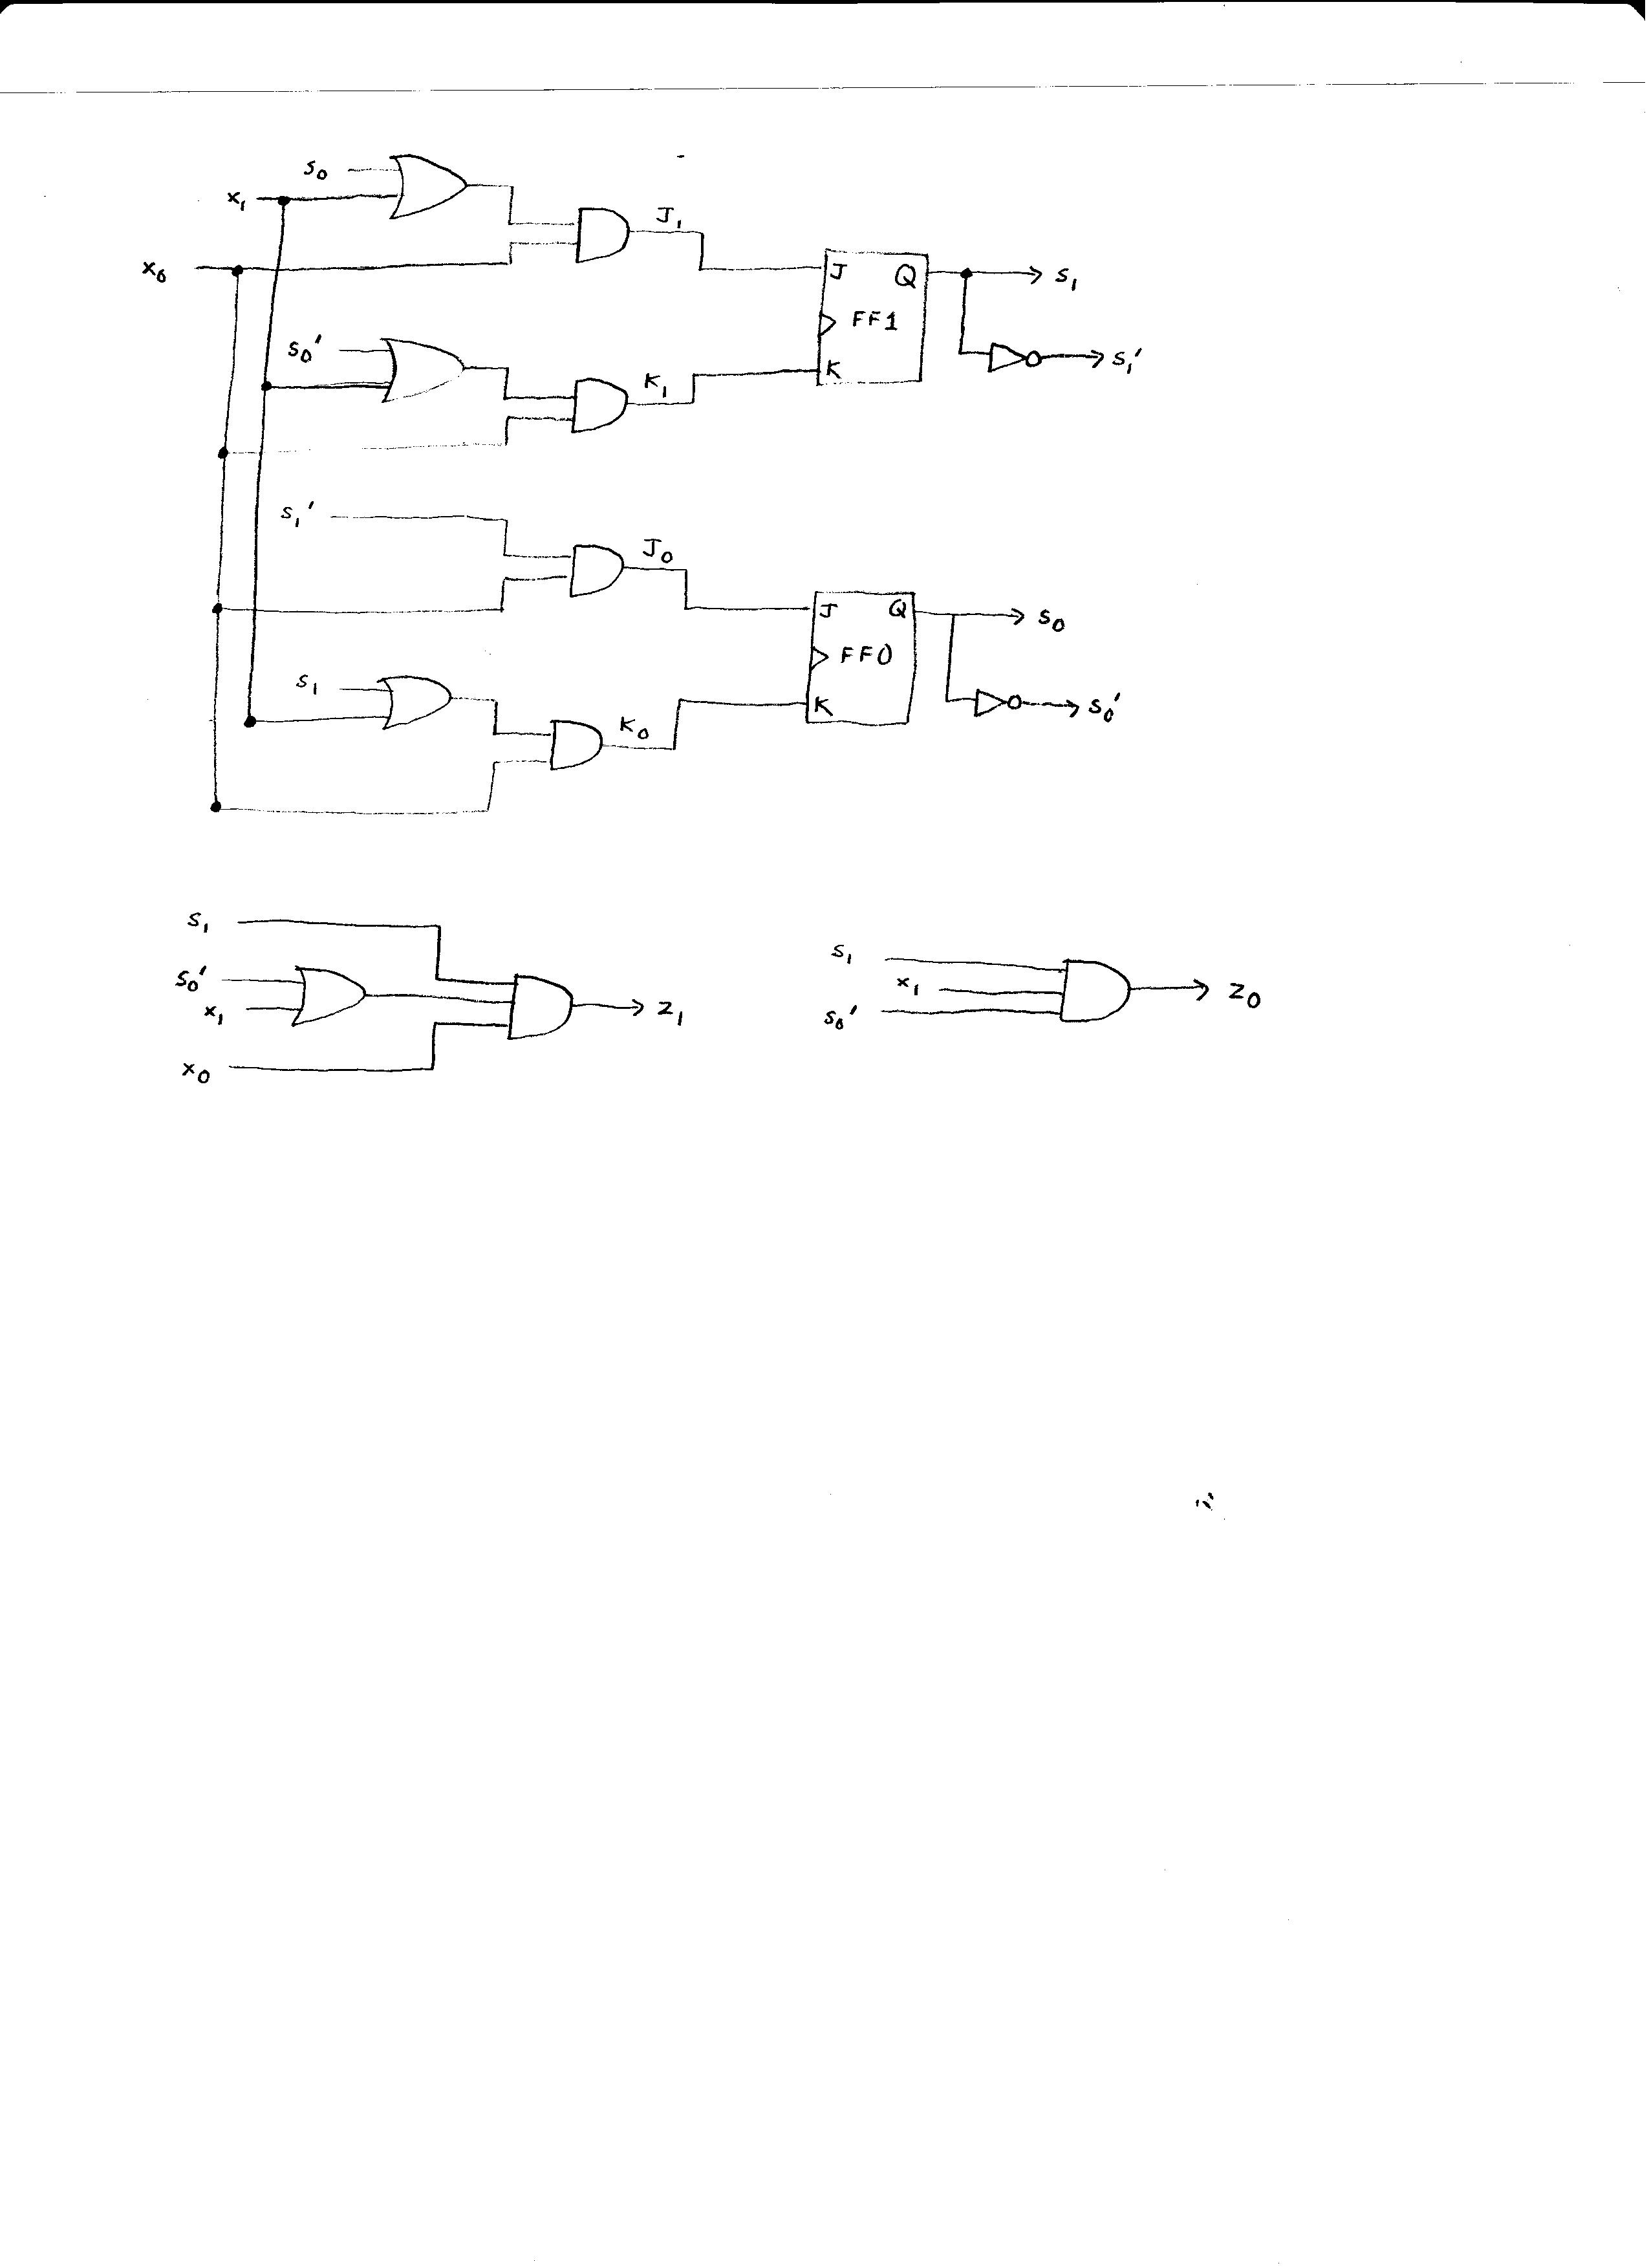
\includegraphics[scale=0.5]{Worksheet(1)}
\caption{First page of our work}
\end{figure}

\begin{figure}[h!]
\centering
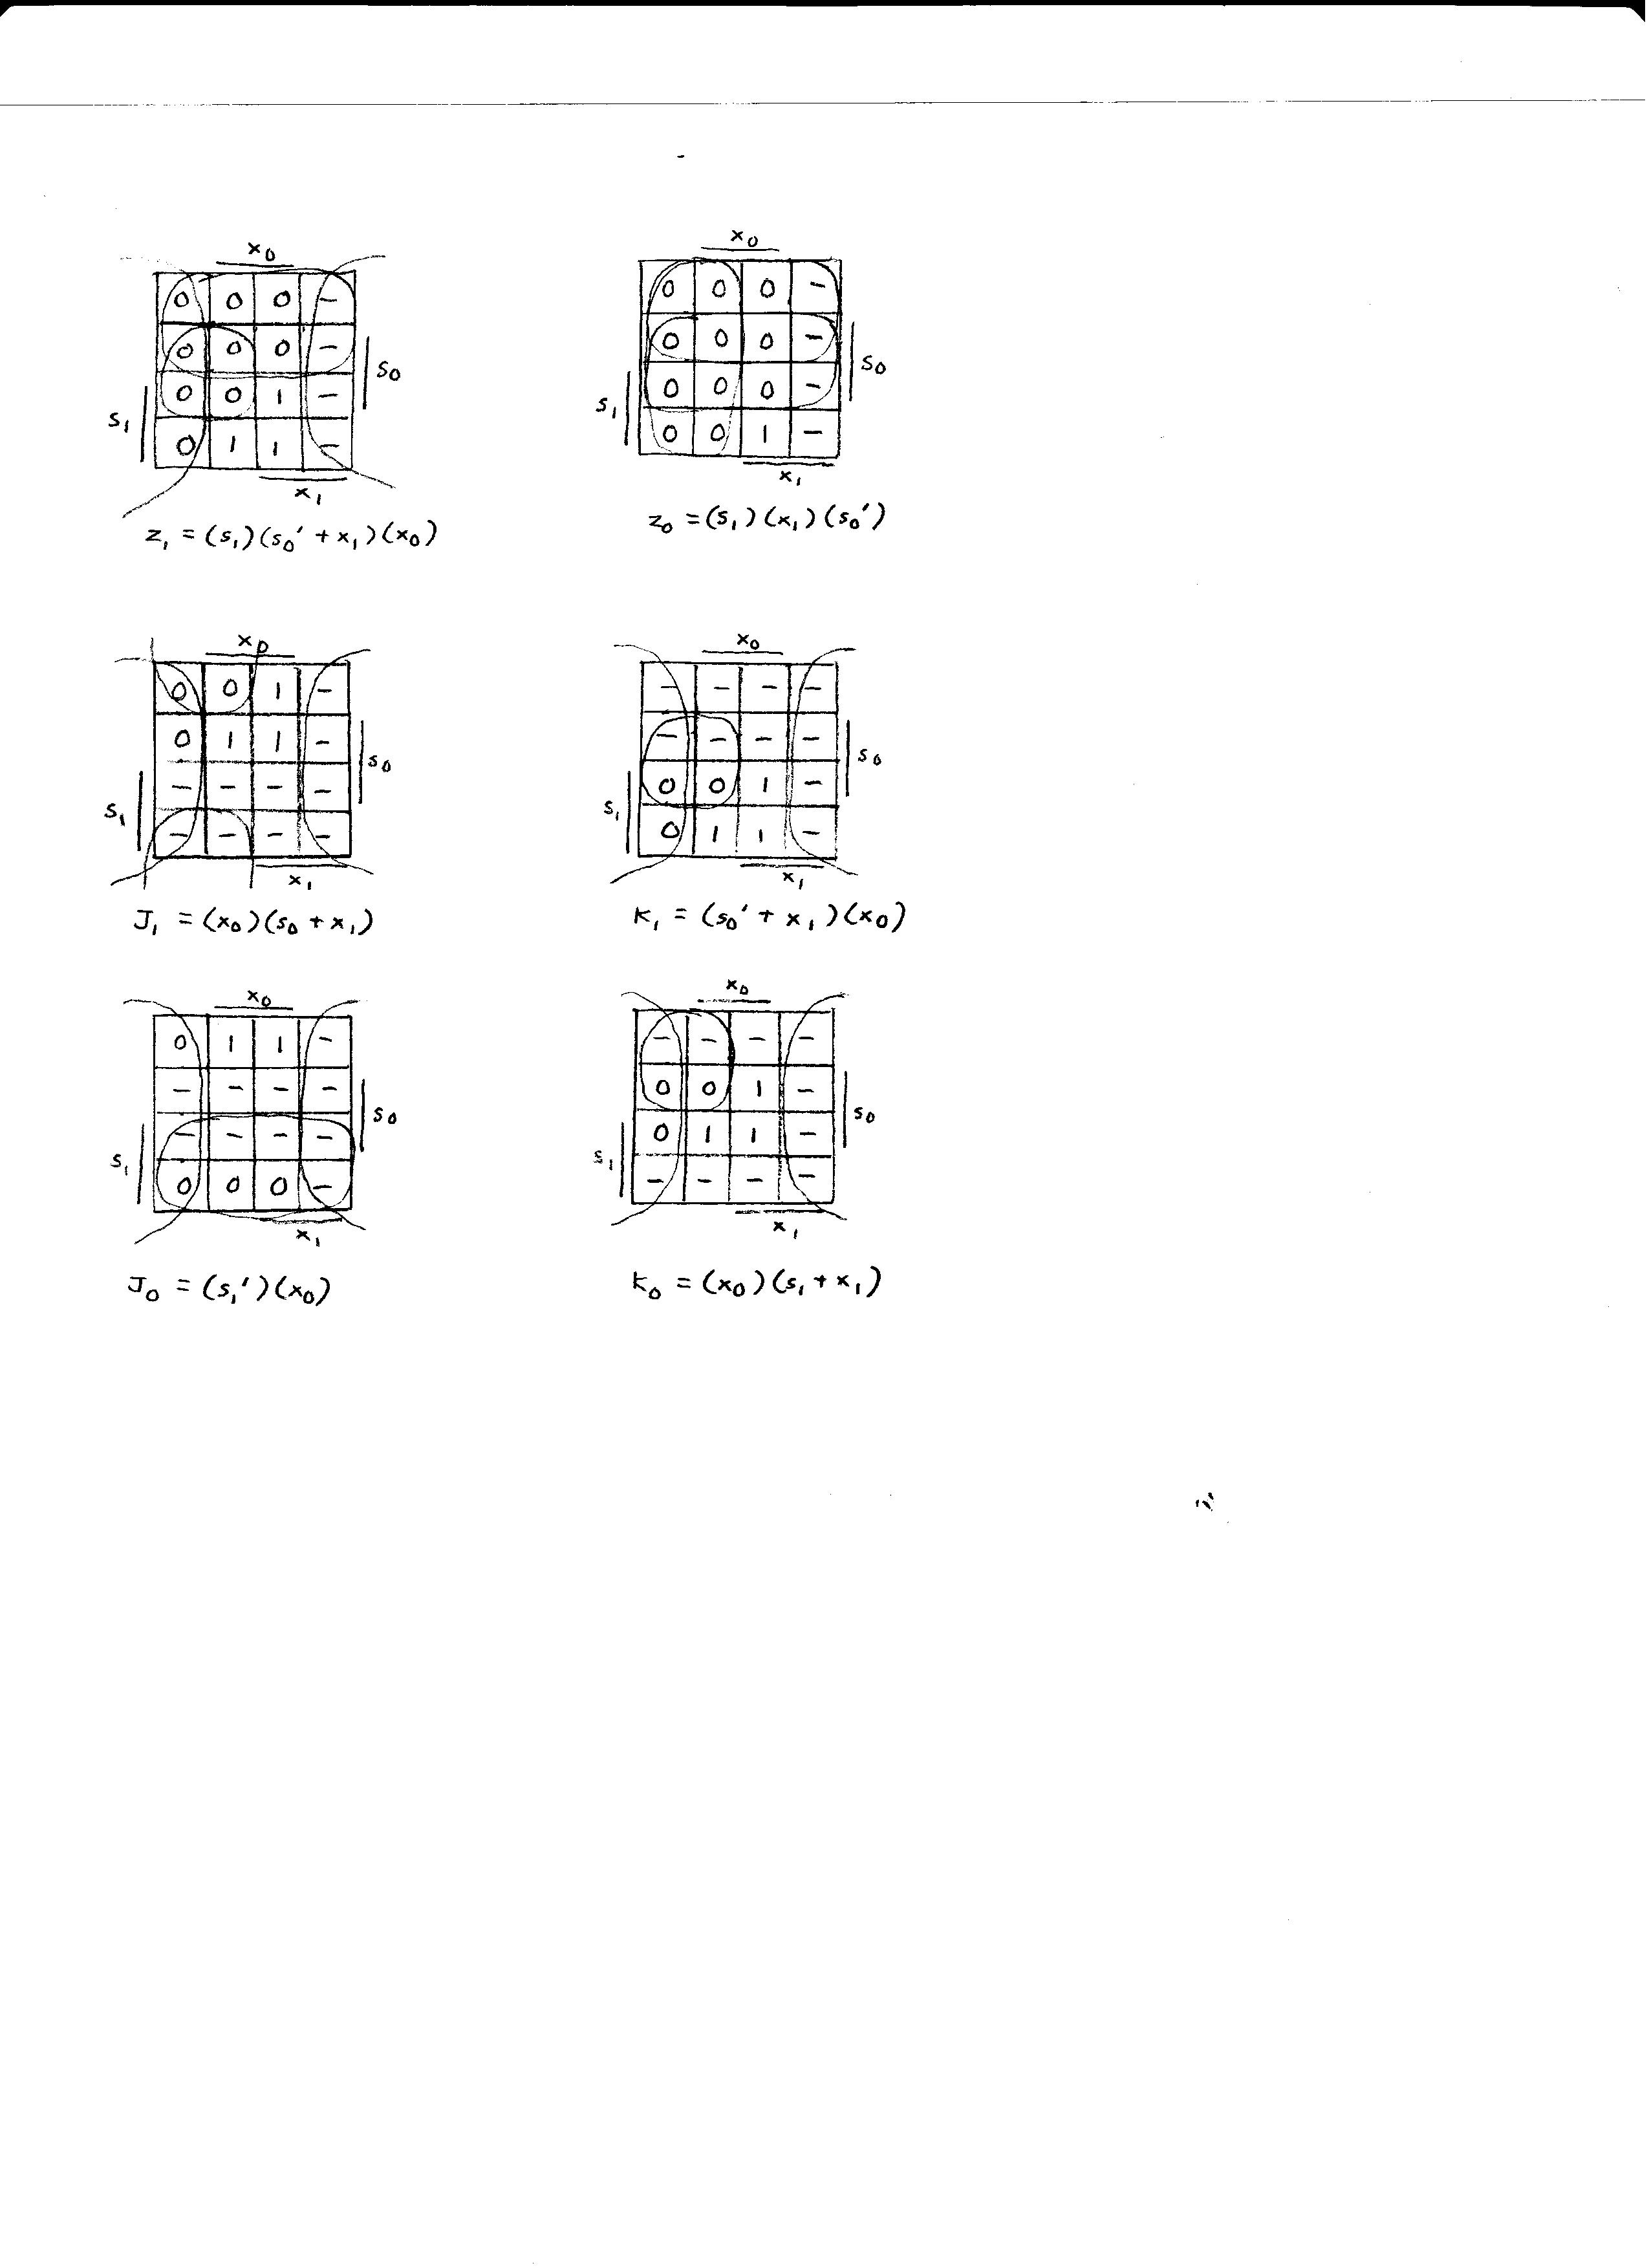
\includegraphics[scale=0.5]{Worksheet(2)}
\caption{Second page of our work}
\end{figure}

%----------------------------------------------------------------------------
\end{document}